\section{Prosthetic Control}

Throughout the development of myoelectric prosthetics, different control schemes have been derived, tested and some implemented in commercially available devices. Complexity and dexterity are dependent on the control system and before choosing a method one must form an overview of the opportunities each presents. The following section will present fundamental concepts of the main control methods. 
 
% Switch based control 
\subsection{Direct switch-based myoelectric control}
A Switch-based myoelectric is the conventional control method and is also known as on/off, crisp, binary or bang/bang control. \cite{Geethanjali2016}
Signal preprocessing is simple and the signal is usually only rectified and filtered. Various sub-control schemes exist, which are either based on the EMG-amplitude of one or two channels. The user is able to control one DoF (e.g. open/closed hand), recorded from one channel, by surpassing a lower amplitude threshold for open hand and a higher closed hand. Alternatively the EMG-signal can be recorded from two independent muscles (two channels) and if a threshold is exceeded in one, the prosthesis would move in a predetermined direction. An illustration of both one and two-channel control schemes can be seen in \figref{fig:Sw}. The actuation speed can be at a fixed speed or proportionally to the EMG amplitude. Multiple DoF's can be achieved by switching the DoF-mode by providing a quick mode-switch signal e.g. two quick contractions, or by physically pressing a switch on the prosthesis. \cite{Farina2014,Wurth2014}  The two channel direct switch-based control scheme can be found in the commercially available Michelangelo Hand \cite{Ottobuck2019}. \\  Switch-based is a simplistic, but slow  control approach. Furthermore, it quickly gets impractical and non-intuitive when increasing the number of DoF's to be replaced as the intended movement is unrelated to the acquisition site. Additionally, the methods relies on isolated muscle contractions, sensitivity might me decreased by channel cross-talk and muscle co-activation. \cite{Wurth2014}    
   
   
 \begin{figure}[H] 
 	\centering
 	\subfigure[One channel threshold control.]
 	{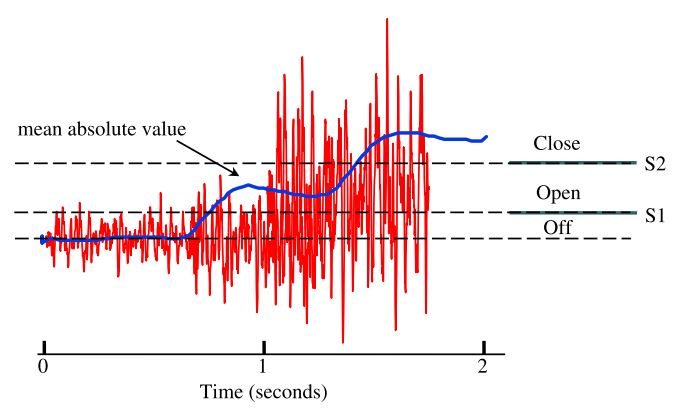
\includegraphics[width=.49\textwidth]{figures/Switch1}}
 	\subfigure[Two channel threshold control.]
 	{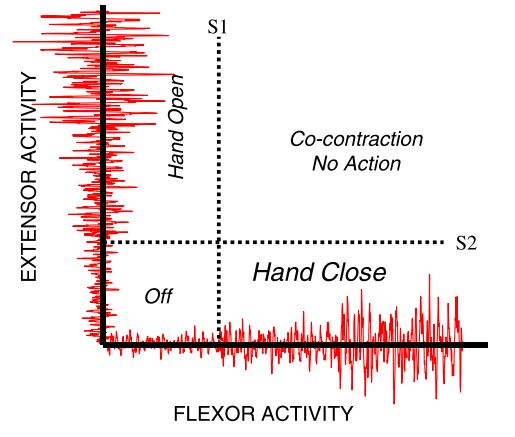
\includegraphics[width=.4\textwidth]{figures/Switch2}}  
 	\caption{Illustration of a direct one channel (a) and two channel (b) threshold control schemes using EMG amplitude to control open/close hand function. S denotes a threshold. Illustration taken from \cite{Parker2006}.}
 	\label{fig:Sw}
 \end{figure}  
   
   
%sequential 
\subsection{Sequential myoelectric control}

To overcome the disadvantages of direct switch-based control in slow and not intuitive control, alternative control strategies relying on algorithms have been derived. Such algorithms could utilize classification-based pattern recognition to predict the intended movement of the user. Often signal from several electrodes are captured. An assumption is that given a consistent movement task is performed the muscles will exhibit a unique activation pattern, and that features extracted from each signal for each movement type can be used to distinguish between different movement types. Hence, complex EMG-signal patterns can be assigned to discrete movement classes, thus also allowing for control of several DoF's.  \cite{Farina2014,Wurth2014}  \\
This approach is more intuitive as it does not demand the need for switching between DoF's, and lowering the amount of effort the user has to put in completing a task. A disadvantage of sequential control is lack of simultaneously controlling multiple DoF's at once allowing for a faster and more natural task execution. \cite{Farina2014}  

%Simultaneous
\subsection{Simultaneous myoelectric control}

Incorporating intuitiveness and naturalness in prosthetic control can be achieved through simultaneous control, where more than one DoF is controlled at a time. Pattern recognition methods predicting more than one movement type have been proposed, but naturalness through proportional actuation speed cannot be achieved independently for each DoF. Instead regression-based methods have been introduced. Compared to classification, which will output one class, trained regressors will continuously output the estimated value for each movement type. Choosing the two movement, which fit the regressors the best will provide simultaneous and proportional control. \cite{Hahne2014} 

